\setcounter{ExampleCounter}{1}
What comes to mind when you think of the word ``average?'' You may think of situations where the average is used: average income, average height, average number of Facebook friends, average test score, etc. The average is a type of center. It tells us the middle of the data. We call the average a \textbf{measure of center}, because it gives a quick snapshot of what a \textit{typical} data point is. But the average is not the only measure of center. In this section, we'll examine several measures of center, how to calculate them and when best to use them.

\subsection{The Mean}
The \textbf{mean} is what most people call the average. To find the mean, you add all the values and divide by the number of values. We can write this in mathematical notation. The Greek letter sigma $\Sigma$ is the symbol for sum. When you see $\Sigma x$, that stands for ``the sum of x.'' The symbol for the mean is $\overline{x}$, read ``x bar.'' Using this information, we can devise a formula for the mean.

\begin{formula}{Mean}
The mean of a sample of size $n$ is
\[\overline{x} = \dfrac{\sum x}{n}.\]

The mean of a population of size $N$ is
\[\mu = \dfrac{\sum x}{N}.\]
\end{formula}

We must note that the symbol for the sample mean is $\overline{x}$, whereas the symbol for population mean is $\mu$ (the lowercase Greek letter, read ``mu'' and pronounced ``mew''). You can assume that the data sets given throughout this section are all samples; hence the mean will be $\overline{x}$.

\begin{example}[https://www.youtube.com/watch?v=CDkM8Hojqg0]{AIDS Patients}
AIDS data indicating the number of months a patient with AIDS lives after taking a new antibody drug are as follows (smallest to largest):
\begin{center}
\begin{tabular}{c c c c c c c c c c}
3 & 4 & 8 & 8 & 10 & 11 & 12 & 13 & 14 & 15\\
15 & 16 & 16 & 17 & 17 & 18 & 21 & 22 & 22 & 24\\
24 & 25 & 26 & 26 & 27 & 27 & 29 & 29 & 31 & 32\\
33 & 33 & 34 & 34 & 35 & 37 & 40 & 44 & 44 & 47\\
\end{tabular}
\end{center}
Calculate the mean.\\

\marginnote{\bfseries Solution}
The calculation for the mean is \[\overline{x} = \frac{3 + 4 + 8 + 8 + 10 + 11 + 12 +...+ 40 + 44 + 44 + 47}{40} = 23.575 \textrm{ months.}\]
To take into account repeated values, we can rewrite the formula. Since the value 8 is repeated twice, instead of using 8+8, we can write (2)(8), and similarly for other repeated values. Hence, we would get\marginnote{Notice that the answer in this alternate solution is rounded to one decimal place.}:\
\[\overline{x} = \frac{3 + 4 + (2)(8) + 10 + ... + 40 + (2)(44) + 47}{40} \approx 23.6 \textrm{ months.}\]
\end{example}
\vfill
\pagebreak

\begin{proc}{Using Your Calculator}
The TI calculator can find the mean for you.
\begin{enumerate}
\item To enter data into the list editor, press \textbf{STAT} then choose option 1:Edit, then enter the data values into list L1.
\item Press \textbf{STAT} and use the arrow button to navigate to the right to the CALC menu. 
\item Choose option 1:1-VarStats. Press the \textbf{2ND} button, then \textbf{1} for list L1. Press \textbf{ENTER}.
\end{enumerate}

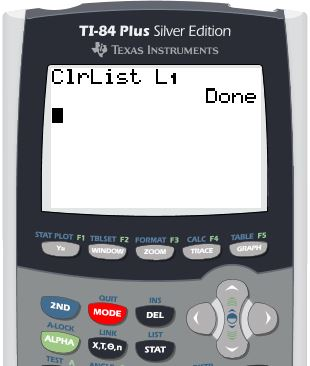
\includegraphics[height=1.5in]{Calc1Sec1_2}
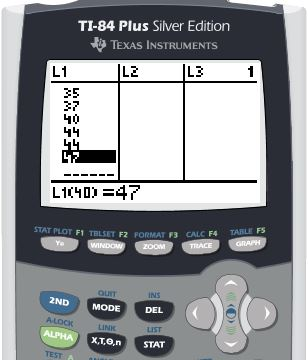
\includegraphics[height=1.5in]{Calc2Sec1_2}
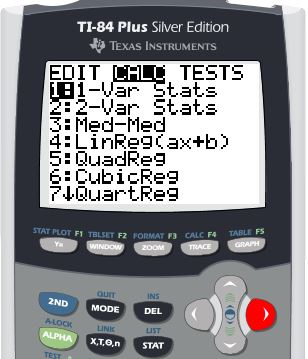
\includegraphics[height=1.5in]{Calc3Sec1_2}
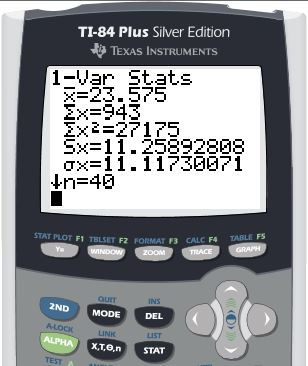
\includegraphics[height=1.5in]{Calc4Sec1_2}
\end{proc}

\begin{try}[http://www.izzomath.com/103text/stats/example2.1/story.html]
The following data show the number of months patients typically wait on a transplant list before getting surgery. Calculate the mean using your calculator.
\begin{center}
\begin{tabular}{c c c c c c c c c c}
3 & 4 & 5 & 7 & 7 & 7 & 7 & 8 & 8 & 9\\
9 & 10 & 10 & 10 & 10 & 11 & 12 & 12 & 12 & 13\\
14 & 14 & 15 & 15 & 17 & 17 & 18 & 19 & 19 & 19\\
21 & 21 & 22 & 22 & 23 & 24 & 24 & 24 & 24
\end{tabular}
\end{center}
\end{try}

The mean can also be calculated from a frequency distribution (as long as it is not grouped).  To illustrate this, consider the following frequency distribution of the data in the example from the previous section about how many hours students worked:
\begin{center}
\begin{tabular}{c | c}
\textbf{Data Value} & \textbf{Frequency}\\
\hline
2 & 3\\
3 & 5\\
4 & 3\\
5 & 6\\
6 & 2\\
7 & 1
\end{tabular}
\end{center}

Recall that this means that there are three 2's, five 3's, and so on.  To calculate the mean, we need to add them all up, but we can do this by multiplying each value by how often it occurs and adding up those results (note that this is exactly what we did at the end of the example about AIDS patients).

\[\overline{x} = \dfrac{2(3)+3(5)+4(3)+5(6)+6(2)+7(1)}{20} = 4.1\]
\vfill
\pagebreak

\subsection{The Median}
We noted at the beginning of this section that we have several measures of center, or ways to describe what a typical data point is.  Why is this necessary?  Since the mean is easy to calculate, why don't we always just use that?

To illustrate why, let's look at the following data set, which shows the income for a sample of 5 people: 
\begin{center}
\begin{tabular}{c c c c c}
\$30,000 & \$45,000 & \$50,000 & \$52,000 & \$1,000,000
\end{tabular}
\end{center}

Calculating the mean for this data set yields \$235,400. Does the mean give a true picture for the center of the data? Can I rightfully say the average person in my data set earns roughly \$235,000? Obviously, the answer is no, since 80\%--or 4/5--of the people in this group earn less than \$53,000. When we have an \textbf{outlier}--a number far removed from the majority of data values--in our data, we should use the median instead of the mean to give a measure of center.

The \textbf{median} is the middle value of a data set when the data is ordered. It is denoted with a capital letter $M$. To find the median, sort the data in order from smallest to largest. If there are an odd number of values in the data set, then the median is the middle value. If there are an even number of values in the data set, then the median is the average or mean of the two middle values.

\begin{example}[https://www.youtube.com/watch?v=KNEKKx8GYHg]{AIDS Patients}
Let's return to our AIDS data set. The data has already been arranged in order from smallest to largest:\begin{center}
\begin{tabular}{c c c c c c c c c c}
3 & 4 & 8 & 8 & 10 & 11 & 12 & 13 & 14 & 15\\
15 & 16 & 16 & 17 & 17 & 18 & 21 & 22 & 22 & 24\\
24 & 25 & 26 & 26 & 27 & 27 & 29 & 29 & 31 & 32\\
33 & 33 & 34 & 34 & 35 & 37 & 40 & 44 & 44 & 47\\
\end{tabular}
\end{center}
Let's find the median.\\

\marginnote{\bfseries Solution}
Since there are an even number of values, we have to take the average of the two middle values. Because there are 40 values, the two middle values are the 20th and 21st values.\begin{center}
\begin{tabular}{c c c c c c c c c c}
3 & 4 & 8 & 8 & 10 & 11 & 12 & 13 & 14 & 15\\
15 & 16 & 16 & 17 & 17 & 18 & 21 & 22 & 22 & {\Large\bfseries 24}\\
{\Large\bfseries 24} & 25 & 26 & 26 & 27 & 27 & 29 & 29 & 31 & 32\\
33 & 33 & 34 & 34 & 35 & 37 & 40 & 44 & 44 & 47\\
\end{tabular}
\end{center}
Here, the 20th and 21st values are both 24. The average of 24 and 24 is 24. So the median is \[M = \textrm{ 24 months.}\]
\end{example}

Note that, like the mean, the units of the median are the same as the original data values.

You can also use the TI Calculator to find the median. The steps are the same as to find the mean; just use the arrow keys to scroll down to the median.
\vfill
\pagebreak

\begin{proc}{Where's the Median?}
To find the median, we want to be able to quickly figure out what position to count to in the ordered data set.  To do this, calculate \[\dfrac{n+1}{2},\] where $n$ is the size of the data set.  Notice that this is the average of 1 and $n$, so it makes sense that this would be halfway between them.
\begin{itemize}
\item If $n$ is odd, $\dfrac{n+1}{2}$ is a whole number.  Count to that position and there you'll find the median.
\item If $n$ is even, $\dfrac{n+1}{2}$ is halfway between two whole numbers.  Find the average of the values at those two positions.
\end{itemize}

For instance, in the example above, $n$ was 40, so we calculated $\dfrac{n+1}{2} = 20.5$, so we knew that the median would be between positions 20 and 21 (the average of the numbers in those positions).
\end{proc}

\begin{try}[http://www.izzomath.com/103text/stats/example2.2/story.html]
The following data shows the number of months patients typically wait on a transplant list before getting surgery. Calculate the median either by hand or using your calculator.
\begin{center}
\begin{tabular}{c c c c c c c c c c}
3 & 4 & 5 & 7 & 7 & 7 & 7 & 8 & 8 & 9\\
9 & 10 & 10 & 10 & 10 & 11 & 12 & 12 & 12 & 13\\
14 & 14 & 15 & 15 & 17 & 17 & 18 & 19 & 19 & 19\\
21 & 21 & 22 & 22 & 23 & 24 & 24 & 24 & 24
\end{tabular}
\end{center}
\end{try}

Just like we did with the mean, we can calculate the median from a frequency distribution.  Let's use the same frequency distribution we did before.
\begin{center}
\begin{tabular}{c | c}
\textbf{Data Value} & \textbf{Frequency}\\
\hline
2 & 3\\
3 & 5\\
4 & 3\\
5 & 6\\
6 & 2\\
7 & 1
\end{tabular}
\end{center}

To find the median, we calculate what position it will occupy in the data set.  Since there are 20 data points, $\dfrac{n+1}{2}=10.5$, so the median will be between the 10th and 11th positions.

If we count through the ordered data set, we go through three 2's, five 3's, and then three 4's, which brings us to the 11th position.  The 10th and 11th positions are both occupied by 4's, so $M=4$.

\paragraph{Outliers:} Let's revisit our income data set:
\begin{center}
\begin{tabular}{c c c c c}
\$30,000 & \$45,000 & \$50,000 & \$52,000 & \$1,000,000
\end{tabular}
\end{center}

The median is \$50,000, which is a more accurate measure of center than the mean. This shows the mean is \textit{sensitive} to outliers, whereas the median is \textit{resistant} to outliers. 

\begin{proc}{Mean and Median}
When outliers are present, the median is a better measure of center. When outliers are absent, the mean can be used.
\end{proc}
\pagebreak

\begin{example}[https://www.youtube.com/watch?v=9H2H_DixDQs]{Siblings} 
A dozen people were asked how many siblings they have. The data is as follows: 
\begin{center}
\begin{tabular}{c c c c c c c c c c c c}
0 & 0 & 1 & 1 & 2 & 2 & 4 & 4 & 5 & 5 & 6 & 6
\end{tabular}
\end{center}
Find the mean and median. Then write a sentence or two explaining why the data values result in those particular mean and median.\\

\marginnote{\bfseries Solution}
The mean is $\overline{x} = 3$ siblings and the median is also $M$ = 3 siblings. This is because there are an equal number of high and low values and they are evenly spaced out.
\end{example}

The sibling data above is called \textbf{symmetric}. Symmetric data is balanced around the mean. A data set is symmetric if the mean and median are roughly equal.

\begin{example}[https://www.youtube.com/watch?v=INc8CRq3JfA]{Salaries}
Suppose that in a small town of 50 people, one person earns \$5,000,000 per year and the other 49 each earn \$30,000. Which is the better measure of the ``center'': the mean or the median?\\

\marginnote{\bfseries Solution}
Since an outlier (\$5,000,000) is present, the median would be a better measure of center.  This is why you'll often find the median salary in a region reported rather than the mean.
\end{example}

When trying to decide whether to use the mean or the median as the measure of the center of a data set, compare them to decide if they are drastically different.  Of course, the best policy is to report both of them and compare them to determine whether the data set is symmetric or \textit{skewed}.

\subsection{The Mode}

There is another, less used, measure of center: the mode. The \textbf{mode} is the most frequently occurring value. There can be more than one mode in a data set as long as those values have the same frequency and the frequency is the highest. A data set with two modes is called \textbf{bimodal}.

\begin{example}[https://www.youtube.com/watch?v=shIDfeUatMU]{Exam Scores}
Statistics exam scores for 20 students are as follows:
\begin{center}
\begin{tabular}{c c c c c c c c c c}
50 & 53 & 59 & 59 & 63 & 63 & 72 & 72 & 72 & 72\\
72 & 76 & 78 & 81 & 83 & 84 & 84 & 84 & 90 & 93
\end{tabular}
\end{center}
Find the mode.\\

\marginnote{\bfseries Solution}
The most frequent score is 72, which occurs five times. \begin{center}Mode = 72.\end{center}
\end{example}

\begin{try}[http://www.izzomath.com/103text/stats/example2.5/story.html]
The number of books checked out from the library from 25 students are as follows: 
\begin{center}
\begin{tabular}{c c c c c c c c c c}
0 & 0 & 0 & 1 & 2 & 3 & 3 & 4 & 4 & 5\\
5 & 7 & 7 & 7 & 7 & 8 & 8 & 8 & 8 & 9\\
10 & 10 & 11 & 11 & 12 & & & & &
\end{tabular}
\end{center}
Find the mode.
\end{try}

The mode can also be observed by looking at a frequency distribution (look for the category with the highest frequency) or a histogram (look for the tallest bar).

\begin{exercises}

\ptwo{Which is the greatest of the following data set: the mean, median or mode?
\[11, 11, 12, 12, 12, 12, 13, 15, 17, 22, 22, 22\]}
\ptwo{Which is the greatest of the following data set: the mean, median or mode?
\[80, 83, 83, 87, 87, 87, 91, 97, 98\]}

\ptwo{One hundred teachers attended a seminar on mathematical problem solving. The attitudes of a representative sample of 12 of the teachers were measured before and after the seminar. The 12 change scores are as follows:
\[3, 8, -1, 2, 0, 5, -3, 1, -1, 6, 5, -2\]
\begin{enumerate}[(a)]
\item What is the mean change score?
\item What is the median change score?
\item What is the best measure of center for this data set: the mean or the median? Why?
\end{enumerate}
}
\ptwo{The following are the amounts of total fat (in grams) in different kinds of sweet treats available at your local donut shop:
\begin{align*}16, 17, 16, 13, 15, 17, 16, 14, 15, 17,\\ 18, 18, 16, 16, 15, 20, 22, 19, 25, 15, 15.\end{align*}
\begin{enumerate}[(a)]
\item What is the mean amount of fat?
\item What is the median amount of fat?
\item What is the best measure of center for this data set: the mean or the median? Why?
\end{enumerate}
}

\ptwo{In a neighborhood donut shop, one type of donut has 530 calories, three types of donuts have 330 calories, four types of donuts have 320 calories, seven types of donuts have 410 calories, and five types of donuts have 380 calories. Find the mean and median calories of the donuts.} 
\ptwo{In a recent issue of \textit{IEEE Spectrum}, 84 engineering conferences were announced. Four conferences lasted 2 days, 36 lasted 3 days, 18 lasted 4 days, 19 lasted 5 days, 4 lasted 6 days, 1 lasted 7 days, 1 lasted 8 days, and 1 lasted 9 days. Find the mean and median length (in days) of an engineering conference.}

\ptwo{A researcher gathered data on hours of video games played by school-aged children and young adults. She collected the following data: \begin{align*}0, 0, 1, 1, 1, 2, 2, 3, 3, 3,\\ 4, 4, 4, 4, 5, 5, 5, 6, 6, 7,\\ 7, 7, 8, 8, 8, 8, 8, 9, 9, 9,\\ 10, 10, 11, 12, 12, 12, 12, 13.\end{align*}
Find the mean and median number of hours.}
\ptwo{The following are the sizes in square feet of the seventeen new faculty offices in the mathematics department at Frederick Community College: \begin{align*}202, 120, 120, 120, 137, 167, 122, 111, 109,\\ 108, 102, 108, 103, 103, 103, 106, 127.\end{align*}
Find the mean and median square footage.}\\

\textit{In exercises 9--10, find the mean, median, and mode for each data set. If there is no mode, state so.}

\ptwo{83, 83, 87, 80, 91, 87, 97, 98}
\ptwo{1, 1, 2, 2, 2, 2, 3, 3, 3, 4, 5, 5, 5, 5}\\

\textit{In exercises 11--14, find the mean and median. Then write a sentence or two explaining why the data values result in those particular means and medians.}

\ptwo{0, 0, 1, 1, 2, 2, 6, 6, 7, 7, 8, 8}
\ptwo{0, 0, 1, 1, 2, 2, 6, 7, 8}

\ptwo{0, 0, 1, 1, 8}
\ptwo{1, 1, 1, 1, 1, 1, 8}

\ptwo{Fifteen students took a statistics pre-test and post-test. The results are below. Find the mean and median pre-test and post-test scores. Then write a sentence or two about what the mean and median tell you in this case. A score of 28 is considered a perfect score.
\begin{center}
\begin{tabular}{c | c | c}
\textbf{Student} & \textbf{Pre-test} & \textbf{Post-test}\\
\hline
& & \\
1 & 9 & 22 \\
2 & 11 & 28 \\
3 & 9 & 18 \\
4 & 4 & 24 \\
5 & 10 & 25 \\
6 & 11 & 16 \\
7 & 9 & 19 \\
8 & 9 & 20 \\
9 & 7 & 18 \\
10 & 8 & 14 \\
11 & 5 & 16 \\
12 & 15 & 26 \\
13 & 12 & 21 \\
14 & 0 & 14 \\
15 & 9 & 13
\end{tabular}
\end{center}
}
\ptwo{Below are the ages and salaries (in thousands of dollars) for CEOs of small companies. Find the mean and median age and salary. Then write a sentence or two about what the mean and median tell you. Data from: http://lib.stat.cmu.edu/DASL/Datafiles/ceodat.html.
\begin{center}
\begin{tabular}{c | c | c}
\textbf{CEO} & \textbf{Age} & \textbf{Salary}\\
\hline
& & \\
1 & 53 & 145 \\
2 & 43 & 621 \\
3 & 33 & 262 \\
4 & 45 & 208 \\
5 & 46 & 362 \\
6 & 55 & 424 \\
7 & 37 & 300 \\
8 & 41 & 339 \\
9 & 55 & 736 \\
10 & 36 & 291 \\
11 & 45 & 58 \\
12 & 55 & 498 \\
13 & 50 & 643 \\
14 & 49 & 390 \\
15 & 47 & 332 \\
16 & 69 & 750
\end{tabular}
\end{center}
}

\pone{In a fifth-grade class, the teacher was interested in the average age of her students. The following data are the ages of a sample of 20 fifth-graders. The ages are rounded to the nearest half-year. Find the average age for this sample: \[9, 9.5, 9.5, 10, 10, 10, 10, 10.5, 10.5, 10.5, 10.5, 11, 11, 11, 11, 11, 11, 11.5, 11.5, 11.5.\]}
\pone{An experiment compared the ability of three groups of participants to remember briefly-presented chess positions. The data are shown below. The numbers represent the number of pieces correctly remembered from three chess positions. Find the mean and median for each group. Then explain what the mean and median tell you about each group's ability to correctly remember chess positions.
\begin{center}
\begin{tabular}{l c c c c c c c c c c}
Non-players: & 22.1 & 22.3 & 26.2 & 29.6 & 31.7 & 33.5 & 38.9 & 39.7 & 43.2 & 43.2\\
Beginners: & 32.5 & 37.1 & 39.1 & 40.5 & 45.5& 51.3 & 52.6 & 55.7 & 55.9 & 57.7\\
Tournament players: & 40.1 & 45.6 & 51.2 & 56.4 & 58.1 & 71.1 & 74.9 & 75.9 & 80.3 & 85.3
\end{tabular}
\end{center}}
\end{exercises}
\pagebreak
